\documentclass{standalone}
\usepackage{tikz}
\usetikzlibrary{arrows.meta,decorations.pathmorphing}

\begin{document}

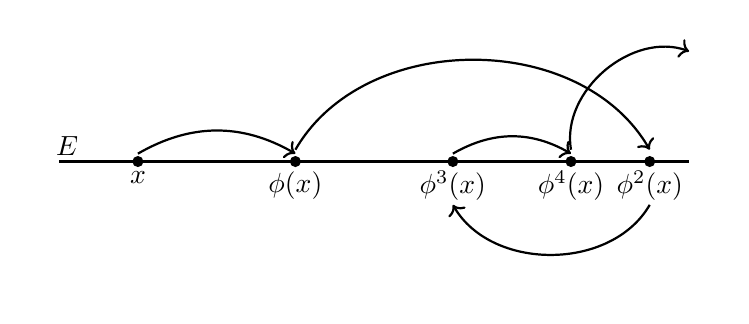
\begin{tikzpicture}
 % Define un área de bounding box para que no cambie el tamaño de la figura
    \useasboundingbox (-1.4,-1.7) rectangle (7.4,1.7);
    % Eje horizontal
    \draw[thick] (-1,0) -- (7,0);

 % Puntos y etiquetas manualmente
    \fill (0,0) circle (2pt);
    \node[below] at (0,0) {$x$};

    \fill (2,0) circle (2pt);
    \node[below] at (2,0) {$\phi(x)$};

    \fill (4,0) circle (2pt);
    \node[below] at (4,0) {$\phi^3(x)$};

    \fill (5.5,0) circle (2pt);
    \node[below] at (5.5,0) {$\phi^4(x)$};

    \fill (6.5,0) circle (2pt);
    \node[below] at (6.5,0) {$\phi^2(x)$};
    
    % Puntos en el eje
    % \foreach \x/\label in {
    % 0/{$x$}, 
    % 2/{$\phi(x)$}, 
    % 4/{$\phi^3(x)$}, 
    % 5.5/{$\phi^4(x)$}, 
    % 6.5/{$\phi^2(x)$}
    % } {
    %     \fill (\x,0) circle (2pt);
    %     \node[below] at (\x,0) {\label};
    % }
    
    % Flechas
    \draw[->, thick] (0,0.1) to[bend left=30] (2,0.1);
    \draw[->, thick] (4,0.1) to[bend left=30] (5.5,0.1);
    \draw[->, thick] (2,0.15) to[bend left=60] (6.5,0.15);
    \draw[->,  thick] (6.5,-0.55) to[bend left=60] (4,-0.55);
    \draw[->,  thick] (5.5,0.15) to[bend left=60] (7,1.4);

 \node at (-0.9, 0.2) {$E$};
    % Flechas finales
    % \draw[->, thick] (6.5,0.1) to[bend left=30] (7.5,0.1);
    % \node[below] at (7.5,0) {$\phi^5(x)$};

\end{tikzpicture}

\end{document}
